\documentclass{beamer}

\usetheme{cambridge}

% Standard packages

\usepackage[english]{babel}
\usepackage[version=4]{mhchem}
%\usepackage{times}
%\usepackage[T1]{fontenc}

%\usepackage{fontspec}
%\setsansfont{Myriad Pro}
%\usefonttheme{professionalfonts}

% Setup TikZ

\usepackage{tikz}
\usetikzlibrary{arrows}

%define a few extra symbols
\tikzstyle{block}=[draw opacity=0.7,line width=1.4cm]
\def \hatH {{\skew4\hat{H}}}
\def \hatA {{\skew6\hat{\cal A}}}
\newcommand{\ah}[2] {\skew2\hat{a}_{\vphantom{b}#1}^{#2}}
\newcommand{\ab}[1] {\skew2\hat{a}_{\vphantom{b}\bf #1}}
\def\hatT{\skew3\hat{T}}
\def\hatC {\skew4\hat{C}}
\def \degrees {$^\circ$}
% These are for non-serif fonts
%\def \hatH {{\skew5\hat{H}}}
%\def \hatA {{\skew5\hat{\cal A}}}
%\newcommand{\ah}[2] {\skew3\hat{a}_{#1}^{#2}}
%\newcommand{\ab}[1] {\skew3\hat{a}_{\bf #1}}
%\def\hatT{\skew4\hat{T}}
\newcommand{\dbd}[2] {{\frac{\partial #1}{\partial #2}}}
\newcommand{\braket}[3] {{\langle #1 | #2 | #3 \rangle}}
\newcommand{\brakett}[3] {{\{ #1 | #2 | #3 \}}}
\newcommand{\brket}[2] {{\langle #1 | #2  \rangle}}
\newcommand{\brkett}[2] {{\{ #1 | #2  \}}}
\newcommand{\bket}[1] {{\langle #1  \rangle}}
\newcommand{\D}[1] {D_{\bf #1}}
\newcommand{\ket}[1] {{| #1 \rangle}}
\newcommand{\kD}[1] {\ket{\D{#1}}}
\def\kDz{\ket{D_0}}
\def\bfr{{\bf r}}
\newcommand{\Or}[1] {${\cal O}$[#1]}
\def\PsiCC{\Psi_{\rm CC}}
\def\PsiCI{\Psi_{\rm CI}}
\newcommand{\up}[2] {{^{#1}\!#2}}
\def\hE{\tilde{E}}


% Author, Title, etc.

\title[Holomorphic Hartree--Fock Theory]
{%
  Holomorphic Hartree--Fock Theory
}
\subtitle{The Thom Group: Theory RIG}

\author[Burton, Thom]
{
  \hskip-1.7mm
  Hugh~Burton %\and
}

\institute[Burton and others]
{
%  \inst{1}%
  University of Cambridge
%  \and
%  \vskip-2mm
%  \inst{2}%
%  Bar-Ilan University, Ramat-Gan, Israel
}

\date[December 2016]{Monday 19th December 2016}

% The main document

\begin{document}

\begin{frame}
  \titlepage
\end{frame}

\begin{frame}{Outline}
  \tableofcontents
\end{frame}

\section{Revision:}

\subsection{Self--Consistent Field Method}
\begin{frame}{Self--Consistent Field Method}
 \begin{itemize}
  \item Begin with set of real orthonormal basis functions $\eta_\mu (\mathbf{r})$.
  \item Construct orthonormal molecular orbitals $\psi_i(\mathbf{r}) = \sum_\mu^n \eta_\mu (\mathbf{r}) C_{\mu i}$.
  \item Form one--particle density matrix $P_{\mu\nu}=\sum_i^N C_{\mu i} (C_{\nu i})^{*}$.
  \item Energy is a functional of density;
  $$E(P_{\mu\nu}) = h_{nuc} + \sum_{\mu\nu}^N P_{\mu\nu} h_{\mu\nu} + \frac{1}{2} \sum_{\mu\nu\sigma\tau}^N P_{\mu\nu} P_{\sigma\tau} \left(2\left(\mu\nu|\sigma\tau\right) - \left(\mu\tau|\sigma\nu\right)\right)$$.
  \item Optimal orbitals are given by $\dbd{E}{P_{\mu\nu}}=0$.
 \end{itemize}
\end{frame} 

\begin{frame}{SCF Solutions to \ce{H2} STO-3G}
  \begin{center}
    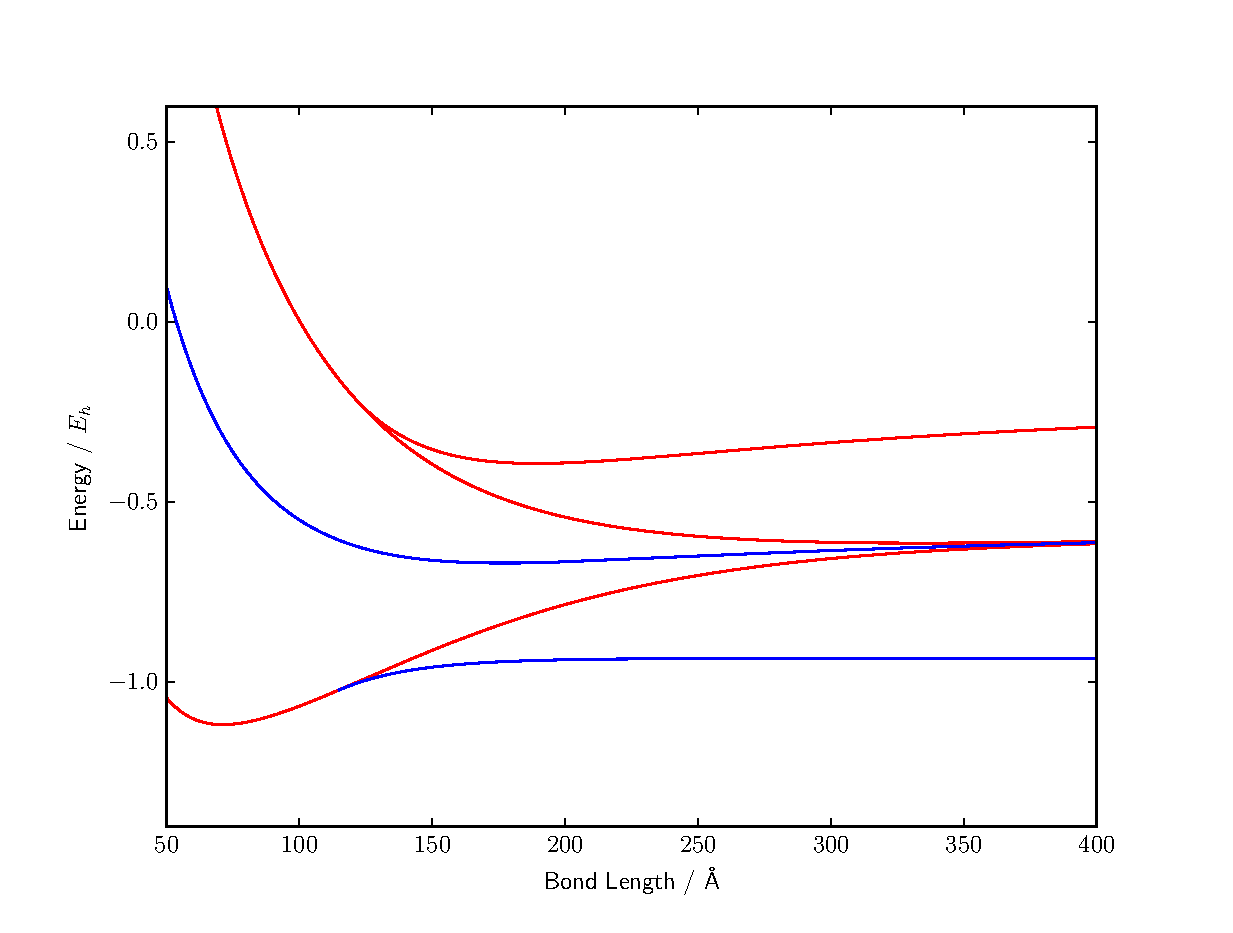
\includegraphics[scale=0.4]{normal_UHF_HH_sto-3g}
  \end{center}
\end{frame}

\subsection{NOCI}
\begin{frame}{Non--Orthogonal CI}
SCF states are size--extensive and could be a basis for CI methods:
\vspace{1em}
 \begin{itemize}
  \item Different SCF solutions ($\up{x}{\Psi}$ and $\up{y}{\Psi}$) are \alert{not orthogonal}.
  \item Solve the generalized eigenvalue problem ${\bf H v}=E{\bf S v}$.
  \item Hamilton matrix elements are given by $H_{xy}=\braket{\up{x}\Psi}{\hat H}{\up y\Psi}$.
  \item Overlap matrix elements are given by $S_{xy}=\brket{\up{x}\Psi}{\up y\Psi}$.
  \item Scales as $\mathcal{O}\left( n_s^2\ \mathrm{max}\left(n^3, N^2\right) \right).$
 \end{itemize}
 \vspace{0.5em}
   \begin{center} 
BUT the number of SCF solutions is \alert{not constant}!!!
  \end{center}
\vspace{0.5em} 
{\tiny A. J. W. Thom and M. Head-Gordon, {\it J. Chem. Phys.} {\bf 131} 124113-1--5, (2009)}
\end{frame}

\begin{frame}{NOCI for \ce{H2} STO--3G}
  \begin{center}
  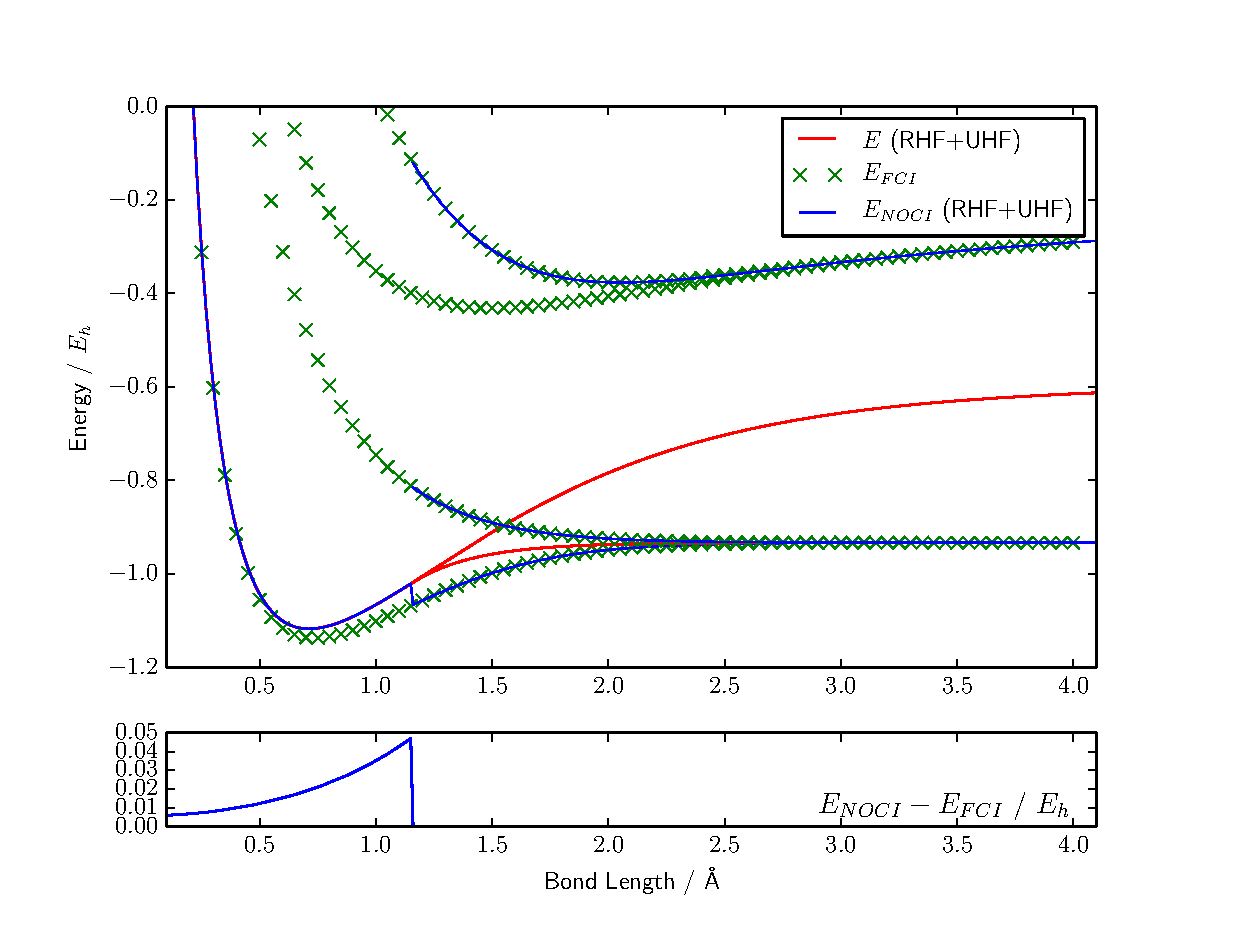
\includegraphics[scale=0.4]{H2_normal}
  \end{center}
\end{frame}

\subsection{Holomorphic HF}
\begin{frame}{Holomorphic Hartree--Fock Theory}
\uncover<1->{\begin{small}
  \begin{quote}
   ``Every non-zero, single-variable, \alert{degree $n$} polynomial with complex coefficients has, counted with multiplicity, exactly \alert{$n$ roots}.''
  \end{quote}
\end{small}
Can we apply this to $\frac{dE}{d\bf P}=0$?} 
\begin{itemize}
  \item<2->{Must be single-variable polynomial $z$}
  \item<2->{Must have no dependence on $z^*$, but $E(P_{\mu \nu})$ depends on $C_{\mu i}^*$.}
 \end{itemize}
 \uncover<2->{Remove dependence on $C_{\mu i}^*$ by defining $\tilde{E}=\frac{\braket{\Psi^*}{\hat H}{\Psi}}{\brket{\Psi^*}{\Psi}}$}
\end{frame}

\begin{frame}{Holomorphic energy functional}
 \uncover<1->{Redefine our energy functional as:
 $$\tilde{E}=\frac{\braket{\Psi^*}{\hat H}{\Psi}}{\brket{\Psi^*}{\Psi}}$$}
\uncover<2->{ Now a holomorphic function of several complex variables $C_{\mu i}$}.
 \begin{itemize}
  \item<3-> $\tilde{E}$ is now in general complex.
  \item<4-> Orbitals must be complex--normalised $\sum_{\mu} C_{\mu \cdot} C_{\mu \cdot} = 1.$
  \item<5-> Density matrix now complex--symmetric $\tilde{P_\mu \nu} = \sum_i^N C_{\mu i} C_{\nu i}$.
 \end{itemize}
 \vfill
 \vspace{2em}
 \uncover<1->{\tiny H. G. Hiscock and A. J. W. Thom, {\it J. Chem. Theory Comput.} {\bf 10} 4795--4800,(2014)}
\end{frame}

\section{Case Study: HZ STO-3G}
\begin{frame}{A simple case study: \ce{HZ}\ \ STO--3G}
\begin{itemize}
 \item<1->{Two electrons in two basis functions (e.g. \ce{H2} - STO-3G).\\ }
 \item<2->{Points on \textit{standard} Grassmannian represented by one parameter:
 $$ \mathbf{C}(z) = \left(
  \begin{matrix}
  \cos z \\  \sin z
  \end{matrix} \right). $$\\ }
 \item<3->{Extend to $\mathbb{C}-$Orthogonal Grassmannian by taking $z = \theta + i \phi$:\\ 
  $$ \mathbf{C}(\theta, \phi) = \left(
  \begin{matrix}
  \cos \theta \cosh \phi - i \sin \theta \sinh \phi \\  
  \sin \theta \cosh \phi  + i \cos \theta \sinh \phi
  \end{matrix} \right). $$}
 \end{itemize}
\end{frame}

\begin{frame}{A simple case study: \ce{HZ}\ \ STO--3G}


\end{frame}

\begin{frame}{\ce{H2} STO-3G*}
 \vspace{-1em}
 \begin{center}

 \end{center}
 \uncover<1->{\tiny H. G. Hiscock and A. J. W. Thom, {\it J. Chem. Theory Comput.} {\bf 10} 4795--4800, (2014)}
\end{frame} 

\begin{frame}{\ce{H2} 6-31G*}
 \vspace{-1em}
 \begin{center}

 \end{center}
 \uncover<1->{\tiny H. G. A. Burton and A. J. W. Thom, {\it J. Chem. Theory Comput.} {\bf 12} 167--173, (2016)}
\end{frame} 







\section{Geometric Approach:}
\subsection{Geometric description of Hartree--Fock}
\begin{frame}{A Geometric Approach: ``Standard'' Hartree--Fock}
\uncover<1->{Optimal set of orbitals given by 
$\psi_i(\mathbf{r})=\sum_\mu^n\eta_\mu(\mathbf{r}) C_{\mu i}.$  }
\begin{itemize}
  \item<1-> $\mathbf{C}$ must be element of unitary group:
  $$\mathrm{U} \left( n \right) = \{ \mathbf{M} \in \mathbb{C}^{n \times n} | \mathbf{M}^{\dagger} \mathbf{M} = \mathbf{I} \}.$$
\end{itemize}
\vspace{-1em}
\uncover<2->{Energy depends on density matrix $P_{\mu\nu}=\sum_i^N C_{\mu i} (C^{\dagger})_{i \nu}$}
\begin{itemize}
  \item<2-> Depends only on first $N$ columns of $\mathbf{C}.$
  \item<2-> Invariant to unitary transformations amongst occupied orbitals.
\end{itemize}
\uncover<3->{Suitable matrices are points on the \alert{Grassmann Manifold} $\mathrm{Gr}(n,N):$
\begin{quote}
  The set of all $(n \times N)$ unitary matrices whose columns span the same subspace.
\end{quote}}
\end{frame}

\begin{frame}{A Geometric Approach: Holomorphic Hartree--Fock}
\uncover<1->{Now restrict such that $\mathbf{C}^T \mathbf{C} = \mathbf{I}:$}
\begin{itemize}
  \item<1-> $\mathbf{C}$ must be element of $\mathbb{C}$-orthogonal group:
  $$\mathbb{C}\mathrm{O} \left( n \right) = \{ \mathbf{M} \in \mathbb{C}^{n \times n} | \mathbf{M}^{T} \mathbf{M} = \mathbf{I} \}.$$
\end{itemize}
\vspace{-1em}
\uncover<2->{Energy depends on holo-density matrix $\tilde{P}_{\mu\nu}=\sum_i^N C_{\mu i} (C^{T})_{i \nu}$\\}
\begin{itemize}
\item<3-> Suitable matrices are now points on the \alert{$\mathbb{C}$-orthogonal} Grassmann Manifold $\mathbb{C}\mathrm{Gr}(n,N):$
\end{itemize}
\uncover<3->{
\begin{quote}
  The set of all $(n \times N)$ $\mathbb{C}$-orthogonal matrices whose columns span the same subspace.
\end{quote}
}
\end{frame}

\subsection{BFGS Algorithm}
\begin{frame}{BFGS Algorithm}
\uncover<1->{
A quasi--Newton optimization algorithm:}
\begin{itemize}
\item Fit local quadratic using \alert{approximate} (inverse) Hessian and take step to centre.
\item Converge onto \alert{all types} of stationary points.
\item Super linear convergence in vicinity of stationary point.
\end{itemize}
\end{frame}

\begin{frame}{BFGS Algorithm}
\begin{enumerate}
  \item<1-> Take an initial guess $\mathbf{x}_0$ and approximate inverse Hessian $\mathbf{B}_0$.
  \item<1-> Obtain search direction by solving $\mathbf{p}_k = - \mathbf{B}_k \mathbf{g}_k.$
  \item<1-> Take line search to find optimal step length $t_k$.
  \item<1-> Update position: $\mathbf{x}_{k+1} = \mathbf{x}_{k} + t_k \mathbf{p}_{k}.$
  \item<1-> Recompute inverse Hessian using BFGS update:
  $$\mathbf{B}_{k+1} =  \left (\mathbf{I}-\frac { \mathbf{s}_k \mathbf{y}_k^{\dagger}} {\mathbf{y}_k^{\dagger} \mathbf{s}_k} \right ) \mathbf{B}_{k} \left (\mathbf{I}-\frac { \mathbf{y}_k \mathbf{s}_k^{\dagger}} {\mathbf{y}_k^{\dagger} \mathbf{s}_k} \right )+\frac
{\mathbf{s}_k \mathbf{s}_k^{\dagger}} {\mathbf{y}_k^{\dagger} \, \mathbf{s}_k}$$
where $\mathbf{s}_k = \mathbf{x}_{k+1} - \mathbf{x}_{k}$ and $\mathbf{y}_k = \mathbf{g}_{k+1} - \mathbf{g}_{k}.$
\end{enumerate}
\end{frame}

\begin{frame}{Constrained BFGS}
\begin{enumerate}
\item<1->{Compute gradient in tangent space ($\mathbf{C}^T \mathbf{\Delta} = 0$):
$$\mathbf{g}_k = (\mathbf{I} - \mathbf{C}_k \mathbf{C}_k^T)\ \frac{\partial \hE}{\partial \mathbf{C}_k}$$}
\item<1->{Compute search direction ($\mathbf{p}_k = - \mathbf{B}_k \mathbf{g}_k$).}
\item<1->{Minimise $||\mathbf{g}(\mathbf{C})||$ along ``geodesic'' with initial direction $\mathbf{p}_k$:
$$\mathbf{C}(t) = \mathbf{C}_k \mathbf{V} \cos(\mathbf{\Sigma} t)\mathbf{V}^T + \mathbf{U} \sin(\mathbf{\Sigma} t) \mathbf{V}^T$$
where $\mathbf{U \Sigma V}^T$ is the complex SVD of $\mathbf{p}_k$.}
\item<1->{Update position:
$$\mathbf{C}_{k+1} = \mathbf{C}(t_{min}).$$}
\end{enumerate}
  \uncover<1->{\tiny B. Savas and L. Lim, {\it SIAM J. Sci. Comput.}, {\bf 32}, 3352--3393, (2010)\\ A. Edelman, T. A. Arias, S. T. Smith, {\it SIAM J. Matrix Anal. Appl.}, {\bf 20}, 303--353, (1998)}
\end{frame}

\begin{frame}{Constrained BFGS}
6. Update approximate Hessian...
\begin{itemize}
\item<1->{How do we compute $\mathbf{y}_k = \mathbf{g}_{k+1} - \mathbf{g}_{k}$?}
\item<1->{$\mathbf{g}_{k}$ and $\mathbf{g}_{k+1}$ must be evaluated at \alert{same point}.} 

\item<2->{Transport matrix defined as:
$$T(t) = \left[\mathbf{C} \mathbf{V}\ \ \mathbf{V} \right] \left[
 \begin{matrix}
 -\sin(\mathbf{\Sigma} t)\\
  \cos(\mathbf{\Sigma} t)
  \end{matrix} \right] \mathbf{U}^T + (\mathbf{I} - \mathbf{U} \mathbf{U}^T)$$.}
\item<2->{Using parallel transported gradient, $\tau \mathbf{g}_k$, gives $$\mathbf{y}_k = \mathbf{g}_{k+1} - T(t_{min})\mathbf{g}_{k}.$$
  } 
 \end{itemize}
 \uncover<1->{\tiny B. Savas and L. Lim, {\it SIAM J. Sci. Comput.}, {\bf 32}, 3352--3393, (2010)\\ A. Edelman, T. A. Arias, S. T. Smith, {\it SIAM J. Matrix Anal. Appl.}, {\bf 20}, 303--353, (1998)}
\end{frame}

\begin{frame}{Constrained BFGS}
6. Update approximate inverse Hessian...
\begin{itemize}
\item<1->{Must also parralel transport $B_{k}$:
$$\tau \mathbf{B}_k = (\mathbf{I} \otimes T(t_{min}))\ \mathbf{B}_k \ (\mathbf{I} \otimes T(t_{min})^{-1})$$}
\item<1->{Can now compute updated inverse Hessian:
$$\mathbf{B}_{k+1} =  \left (\mathbf{I}-\frac { \mathbf{s}_k \mathbf{y}_k^{\dagger}} {\mathbf{y}_k^{\dagger} \mathbf{s}_k} \right ) \tau \mathbf{B}_{k} \left (\mathbf{I}-\frac { \mathbf{y}_k \mathbf{s}_k^{\dagger}} {\mathbf{y}_k^{\dagger} \mathbf{s}_k} \right )+\frac
{\mathbf{s}_k \mathbf{s}_k^{\dagger}} {\mathbf{y}_k^{\dagger} \, \mathbf{s}_k}.$$}
 \end{itemize}
 \vspace{2em}
 \uncover<1->{\tiny B. Savas and L. Lim, {\it SIAM J. Sci. Comput.}, {\bf 32}, 3352--3393, (2010)}

\end{frame}

\section{Slippery Issues}
\begin{frame}{Future Directions}
 \begin{itemize}
  \item<1->{Currently working to apply geometric optimisation methods on holomorphic energy surface.}
  \item<2->{Hope to understand holomorphic states and the topology of the energy functional.}
  \item<3->{Will investigate the applicability of using NOCI for studying larger molecules.}
  \item<4->{Consider using holomorphic states for other post-HF correlation methods.}
 \end{itemize}
\end{frame}

\begin{frame}{Acknowledgements}
 I would like to thank:
 
 \begin{itemize}
  \item{Alex Thom}
  \item{The Thom Group}
  \item{The Cambridge Trust}
 \end{itemize}
 \begin{center}
  
\includegraphics[scale=0.7]{template/CT_logo.jpg}
 \end{center}
\end{frame}
\end{document}
